% Document Class and Basic Packages
%-------------------------------------------------------------------------------
\documentclass[letterpaper,12pt]{article} % Define the document class and options
\usepackage{graphicx} % For including graphics
\usepackage[margin=1in]{geometry}
\usepackage{cite} % Handle citations
\usepackage[final]{hyperref} % Add hyperlinks
\usepackage{pgfplotstable, booktabs} % Enhance table handling
\usepackage{placeins} % Control float placement
\usepackage{tabularray} % Advanced tables
\usepackage{titlesec} % Customize section titles
\usepackage{fancyhdr} % Create custom page headers and footers
\usepackage{empheq} % Highlight equations
\usepackage{amssymb} % Extended math symbols
\usepackage{tcolorbox} % Colored boxes
\usepackage{enumitem} % Enhanced list environments
\usepackage{xcolor} % Define custom colors
\usepackage{parskip} % Adjust paragraph spacing
\usepackage{siunitx} % Handling SI units
\usepackage{cancel} % Strikethrough text
\usepackage{listings} % Include code listings
\usepackage{tocloft}  % Table of contents formatting
\usepackage{mathtools}
\usepackage{pdfpages}
\usepackage{times}

% 1.5 spacing equivalent to word
\usepackage{setspace}
\linespread{1.25}


% Define Custom Colors
%-------------------------------------------------------------------------------
\definecolor{codegreen}{rgb}{0,0.6,0}
\definecolor{codegray}{rgb}{0.5,0.5,0.5}
\definecolor{codepurple}{rgb}{0.58,0,0.82}

% Define Code Listing Style
%-------------------------------------------------------------------------------
\lstdefinestyle{mystyle}{
    commentstyle=\color{codegreen},
    keywordstyle=\color{codepurple},
    numberstyle=\tiny\color{codegray},
    stringstyle=\color{codegreen},
    basicstyle=\ttfamily\small,
    breakatwhitespace=false,         
    breaklines=true,                 
    captionpos=b,                    
    keepspaces=true,                                                     
    showspaces=false,                
    showstringspaces=false,
    showtabs=false,                  
    tabsize=4
}

\DeclarePairedDelimiter\abs{\lvert}{\rvert}%
\DeclarePairedDelimiter\norm{\lVert}{\rVert}%

% Swap the definition of \abs* and \norm*, so that \abs
% and \norm resizes the size of the brackets, and the 
% starred version does not.
\makeatletter
\let\oldabs\abs
\def\abs{\@ifstar{\oldabs}{\oldabs*}}
%
\let\oldnorm\norm
\def\norm{\@ifstar{\oldnorm}{\oldnorm*}}
\makeatother

% Set Code Listing Style
\lstset{style=mystyle}

% Define Custom Commands and Settings
%-------------------------------------------------------------------------------
\newcommand*\widefbox[1]{\fbox{\hspace{0em}#1\hspace{0em}}} % Create a wide box
\newcommand{\tr}{\text{tr}} % Define a trace command for math mode

% Page Header and Footer Setup
%-------------------------------------------------------------------------------
\pagestyle{fancy} % Use the fancy page style
\fancyhf{} % Clear all header and footer fields
\fancyhead[L]{MEC E 301} % Left-aligned header
\fancyhead[C]{Lab 2: Digital Measurement Techniques} % Center header
\fancyhead[R]{Alex Diep} % Right-aligned header
\fancyfoot[C]{\thepage} % Centered page number in the footer

% Section and Subsection Formatting
%-------------------------------------------------------------------------------
%\titleformat*{\section}{\Large\bfseries} % Customize section titles
%\titleformat*{\subsection}{\large\bfseries} % Customize subsection titles
\renewcommand{\thesection}{Question \arabic{section}} % Modify section numbering
\renewcommand{\thesubsection}{(\alph{subsection})} % Modify subsection numbering

% Hyperlink Setup
%-------------------------------------------------------------------------------
\hypersetup{
	colorlinks=true, % Enable colored links
	linkcolor=blue, % Set link color
	citecolor=blue, % Set citation color
	filecolor=magenta, % Set file link color
	urlcolor=blue % Set URL link color
}

% Indentation Setup
%-------------------------------------------------------------------------------
%\newcommand{\forceindent}{{\setlength{\parindent}{2em}\indent}}

% Custom SI Unit Definitions
\DeclareSIUnit\LSB{LSB} % Least significant bit

% Custom Table of Contents Formatting
\renewcommand\cftsecdotsep{\cftdot} % Use dots for section 
\renewcommand{\cftsecleader}{\cftdotfill{\cftsubsecdotsep}} % Use subsection dots for section

\sisetup{group-digits=false} % changes the default (true)
% \titlespacing\section{0pt}{12pt plus 4pt minus 2pt}{0pt plus 2pt minus 2pt}
% \titlespacing\subsection{0pt}{12pt plus 4pt minus 2pt}{0pt plus 2pt minus 2pt}
% \titlespacing\subsubsection{0pt}{12pt plus 4pt minus 2pt}{0pt plus 2pt minus 2pt}
\titlespacing*{\section}{0pt}{0.1\baselineskip}{0.2\baselineskip}
\titlespacing*{\subsection}{0pt}{0.1\baselineskip}{0.2\baselineskip}
\titlespacing*{\subsubsection}{0pt}{0.1\baselineskip}{0.2\baselineskip}

% End of Preamble
%-------------------------------------------------------------------------------

%++++++++++++++++++++++++++++++++++++++++
\begin{document}
\begin{titlepage}
    \centering
    \vspace*{2cm} % Adjust vertical spacing
    
    % Title
    \Huge {MEC E 301 \\Lab 4: Displacement Transducers} \\
    \vspace{1cm} % Adjust vertical spacing
    
    % Author
    \Large by: Alex Diep \\
    \vspace{1cm} % Adjust vertical spacing

    % Date
    \Large Date: October 19, 2023 (Extension Approved) \\ % or manually specify a date
    \vspace{4cm} % Adjust vertical spacing

    % CCID and Student ID in smaller font
    \normalsize CCID: abdiep \\
    \normalsize Student ID: 1664334 \\ 
    \normalsize Section: D21 \\
    
    \vfill % Fill vertical space
    
    % Additional content (e.g., university logo or other information)
    
\end{titlepage}
\renewcommand\arraystretch{1.5}

% % Table of Contents (Hyperlinks set to locally black)
% {
%     \hypersetup{hidelinks}
%     \tableofcontents
% }
% % use roman numerals for page numbers in table of contents
% \pagenumbering{roman}

% \newpage

% seperate page count for main matter
\pagenumbering{arabic}


% Worksheet
% NOTE: For two marks complete and hand-in Pages 7-8 before the end of the lab.
% You are a design engineer working at a large automotive component manufacturer. You 
% have been asked to design a system to monitor the air intake filter on an engine. You are 
% to devise a system that will determine if the air filter is properly installed or damaged and
% when the filter is clogged, which will turn on the engine warning light, so that the driver 
% knows that the filter will need to be replaced. 
% When a clean filter is installed, the pressure drop across the filter is 0.7 kPa when the 
% engine is at idle. (The pressure drop is the differential pressure between the air upstream 
% and downstream of the filter). If a filter has a leak due to damage or improper installation, 
% then the pressure drop will be lower than 0.7 kPa. For example, the pressure drop will be 
% zero if no filter is installed. Also, as debris is collected on the filter the pressure drop 
% increases. The filter should be replaced when the pressure drop reaches 0.9 kPa when the 
% engine is at idle. Thus, it is desired to measure pressure drops from 0 to 0.9 kPa.
% The analog signal from the pressure transducer will be read by the vehicle’s engine 
% control unit (ECU). The ECU uses a 12-bit A/D converter and accepts 0–5 V input 
% voltage.
% Your supervisor told you to use a sensor from Honeywell (see data sheet posted on 
% eClass) that measures differential pressure with the model number: 
% ABP2 D DA D XXXXX A A Y, where XXXXX is a place holder for the pressure range, 
% and Y is a place holder for the supply voltage (either 3.3 V or 5 V). See Page 10 of the 
% data sheet to understand the model number. 
% Recommend a system to monitor the pressure drop by completing the following steps:
% 1) See Page 10 of the data sheet and select a pressure range in kPa which is 
% suitable for your application. [1 mark]. Why did you choose that range? [1 
% mark].
% 2) See Page 6 of the data sheet. The output of the sensor depends on the supply 
% voltage of the sensor. Plot the expected voltage output of your sensor as a 
% function of pressure over the range of the sensor if the supply voltage is 3.3 V 
% and if it is 5V. Put both lines on the same plot. [2 marks]. Calculate the 
% sensitivity of the sensor for each supply voltage. [1 mark]
% 3) The ECU uses 12-bit A/D converters and has channels which can accept 0–
% 5 V input voltages. Also, it is possible to amplify the signal out of the sensor 
% before it goes to the ECU. For each supply voltage (either 3.3 V or 5 V), 
% calculate the maximum amplification you could use [3 marks] and the 
% resulting resolution of the measurement system in units of kPa [1 marks]
\section{}
% Question 1
Define a list of the design criteria:
\begin{itemize}
    \item Pressure range: 0-0.9 kPa
    \item Resolution should be maximized since the number of bits is fixed to $2^{12}$
    \item Working unit: kPa
\end{itemize}

One pressure range meets these constraints: $\boxed{\text{001KD}}$.   

\section{}
% qeustion 2 reponse
\begin{figure}[h]
    \centering
    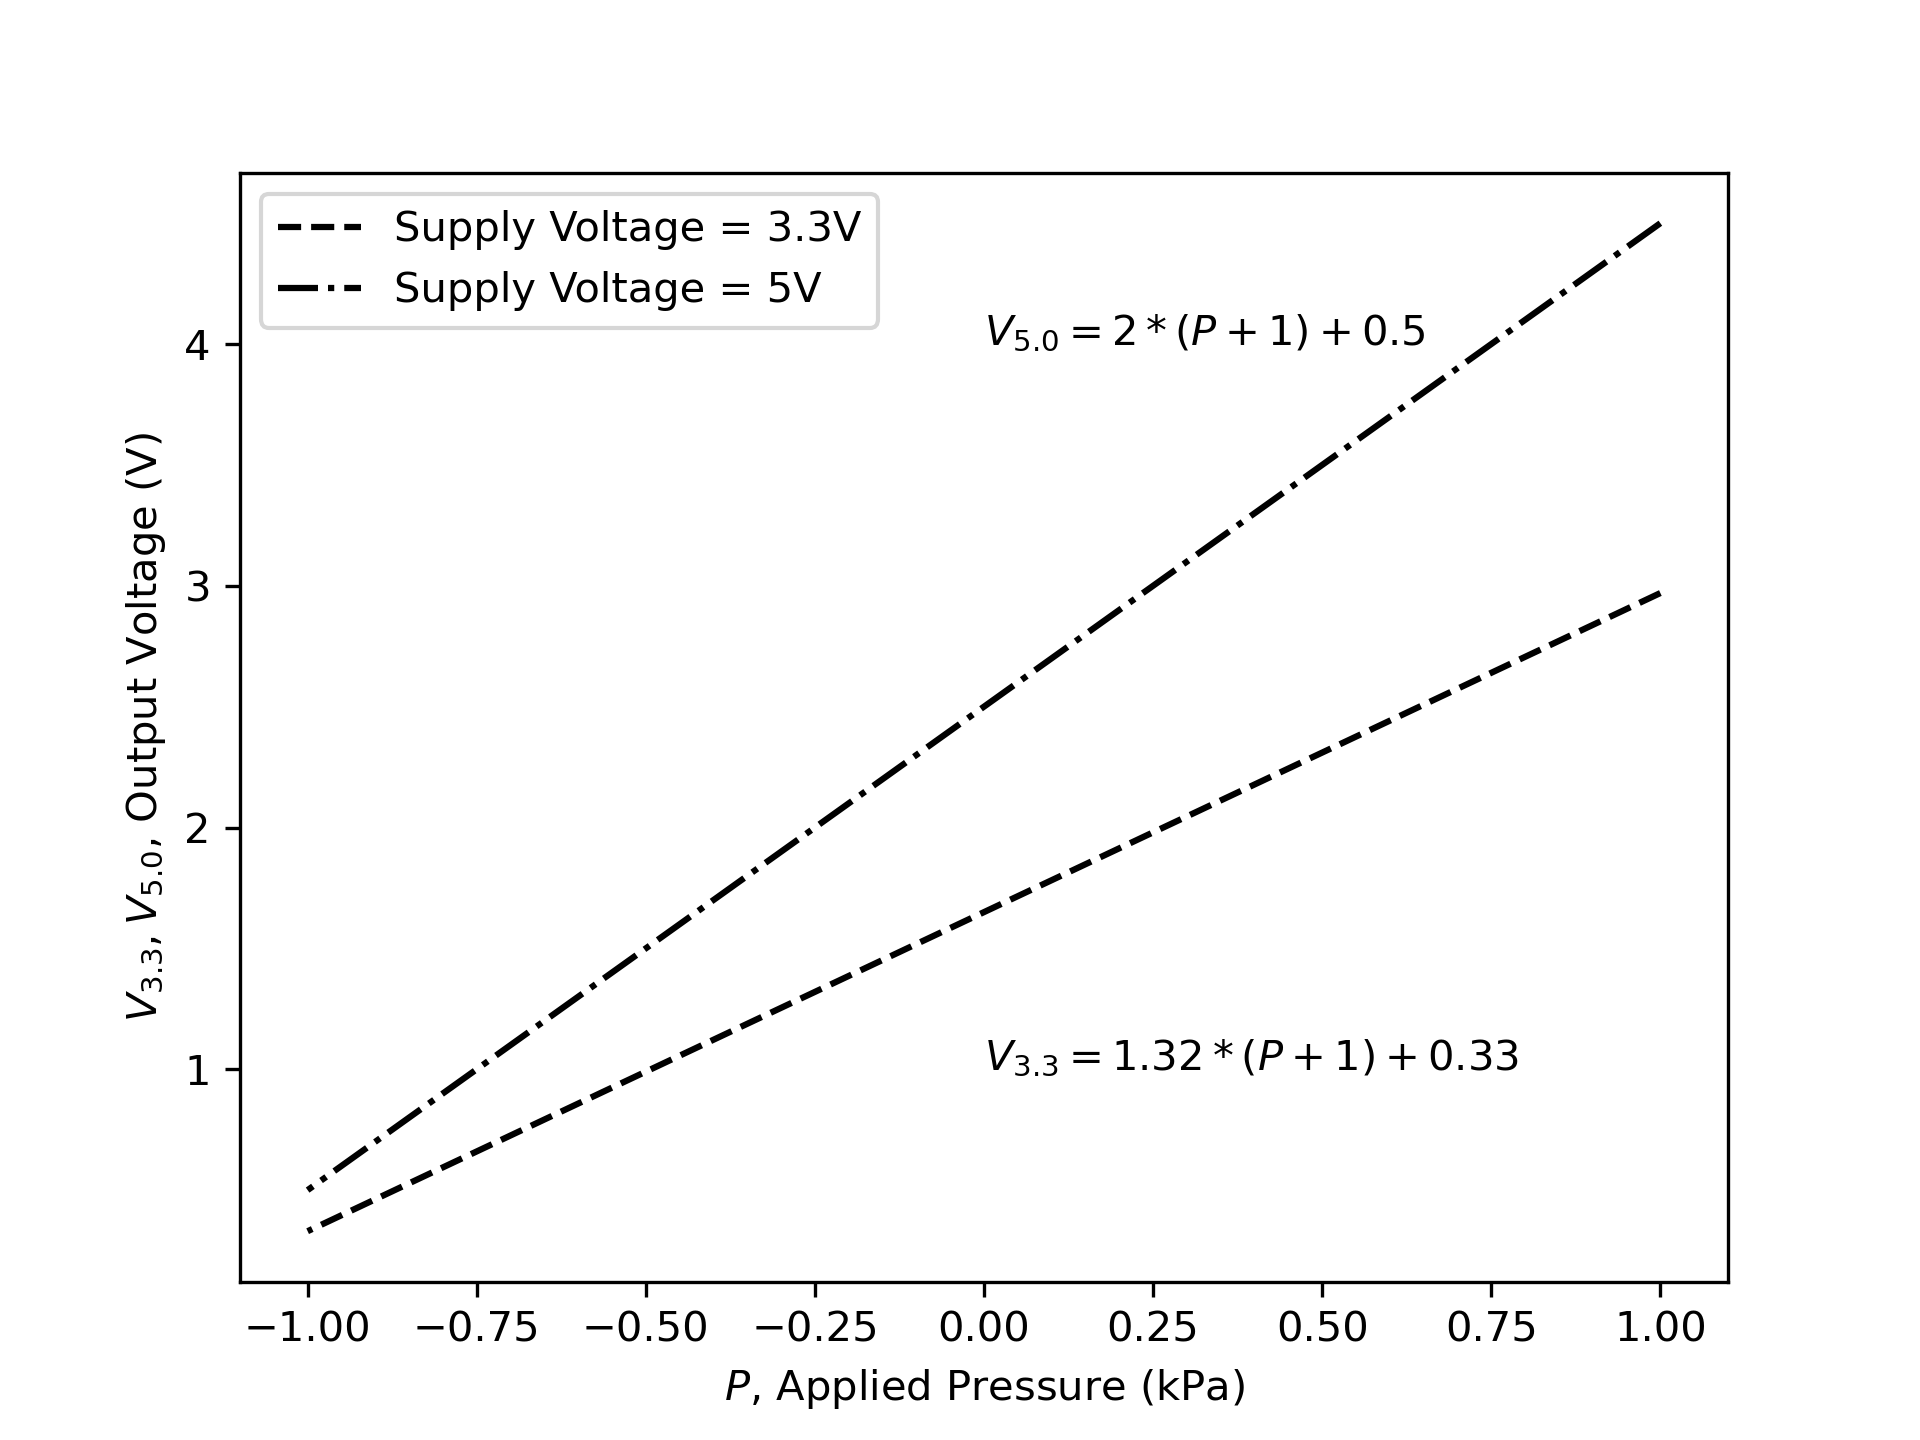
\includegraphics[width=0.8\linewidth]{matplotlib/q2VoltageOutputPlot.png}
    \caption{Voltage output of the sensor as a function of pressure over the range of the sensor if the supply voltage is 3.3 V and if it is 5V.}
    \label{fig:q2VoltageOutputPlot}
\end{figure}
The sensitivity of the sensor for each supply voltage is calculated by taking the derivative of the voltage output with respect to pressure. 
Since the equations for the voltage output are linear, the sensitivity is constant. 
\begin{empheq}[box=\fbox]{align*}
    \text{Sensitivity}_{3.3V} &= \frac{d}{dP} \left(1.32(P+1) + 0.33 \right) = 1.32 \text{ V/kPa} \\
    \text{Sensitivity}_{5V} &= \frac{d}{dP} \left(2(P+1) + 0.5 \right) = 2 \text{ V/kPa}
\end{empheq}

% plt.text(0, 1, '$V_{3.3} = 1.32*(P+1) + 0.33$')
% plt.text(0, 4, '$V_{5.0} = 2*(P+1) + 0.5$')

\section{}
The transfer function being used has an output range of 10\% to 90\% of the input range. That means the maximum output of the 
sensor is $0.9V_{\text{input}}$.

The voltage that the sensor outputs at $0.9$ kPa is not the maximum voltage. Determining that from the equations from Fig. \ref{fig:q2VoltageOutputPlot} gives:
\begin{align*}
    V_{3.3, \text{max}} &= 1.32(0.9+1) + 0.33 = \qty{2.838}{\volt} \\
    V_{5.0, \text{max}} &= 2(0.9+1) + 0.5 = \qty{4.3}{\volt} \\
\end{align*}
These values correspond to the maximum output of the sensor in practice. There is some wiggle room since the EDC can read up to 5V,
\begin{empheq}[box=\fbox]{align*}
    \text{Amplification}_{3.3\text{V}} &= \frac{V_{\text{EDC, max}} - V_{\text{EDC, min}}}{V_{3.3, \text{max}}} = \frac{5 - 0}{2.838} = 1.76 \\
    \text{Amplification}_{5.0\text{V}} &= \frac{V_{\text{EDC, max}} - V_{\text{EDC, min}}}{V_{5.0, \text{max}}} = \frac{5 - 0}{4.3} = 1.16
\end{empheq}
The resolution of the measurement systems are:
\begin{empheq}[box=\fbox]{align*}
    \text{Resolution}_{3.3\text{V}} &= \frac{V_{\text{EDC, max}} - V_{\text{EDC, min}}}{2^{n} G (\text{sensitivity}_{3.3V})} \\
    &= \frac{5 - 0}{2^{12} \times 1.76 \times 1.32} = \qty{5.2e-4}{\kilo\pascal} \\
    \text{Resolution}_{5.0\text{V}} &= \frac{V_{\text{EDC, max}} - V_{\text{EDC, min}}}{2^{12} G (\text{sensitivity}_{5V})} \\
    &= \frac{5 - 0}{2^{12} \times 1.16 \times 2} = \qty{5.2e-4}{\kilo\pascal}
\end{empheq}

\section{}
% 4) Read Page 3 and Page 13 of the data sheet. Determine the total bias 
% uncertainty in your system, in units of kPa, for each supply voltage (either 3.3 
% V or 5 V) using maximum amplification when the pressure transducer is 
% measuring 0.9 kPa when used in the temperature range of -20 to 85 oC. [3 
% marks] [Note: There is a bias uncertainty due to resolution of the A/D and a 
% bias uncertainty of the sensor].
At the operating temperature range of -20 to 85 $^\circ$C, the bias uncertainty of the sensor is $\pm 3.5\%$ FSS (Full Scale Span). Full scale,
as defined by the manufacturer, is the difference between the maximum and minimum output signals at the limits of pressure range.

The total bias uncertainty of the system is the RSS of the two independent uncertainties.

For the 3.3V supply voltage, the bias uncertainty of the sensor is:
\begin{align*}
    \text{Bias Uncertainty}_{3.3V} &= \% \text{err} \times \frac{\text{FSS}}{\text{sensitivity}} \\
    &= \pm 0.035 \times \frac{0.9\times3.3 - 0.1\times3.3}{1.32} = \qty{0.070}{\kilo\pascal}
\end{align*}
For the 5V supply voltage, the bias uncertainty of the sensor is:
\begin{align*}
    \text{Bias Uncertainty}_{5V} &= \% \text{err} \times \frac{\text{FSS}}{\text{sensitivity}} \\
    &= \pm 0.035 \times \frac{0.9\times5 - 0.1\times5}{2} = \qty{0.070}{\kilo\pascal}
\end{align*}

The bias uncertainty in kPa for 3.3V and 5V supply voltages are the exact same. In addition their resolutions are also the exact same. Calculating the
RSS for total uncertainty:
\begin{empheq}[box=\fbox]{align*}
    \delta P_{3.3\text{V}} = \delta P_{5.0\text{V}} &= \sqrt{\text{Quantization Uncertainty}^2 + \text{Bias Uncertainty}^2} \\
    &= \sqrt{(5.2 \times 10^{-4}/2)^2 + (7.0 \times 10^{-2})^2} = \qty{7.0E-2}{\kilo\pascal}
\end{empheq}
Observe that the bias uncertainty is much larger than the resolution of the system, and is the major contributor to the total uncertainty.
\section{}
% 5) State which supply voltage and amplification (if any) that should be used. [1 
% mark]. Is the cost and complexity of amplification worth the benefit of 
% increased resolution? [1 mark]. Why do you recommend the supply voltage 
% that you did? [1 mark] Is the uncertainty acceptable for this application? Why
% or why not? [1 marks]
The unamplified 5.0V system will be used.

The cost and complexity of amplification is not worth the small increased resolution. Additionally, the amplifier will introduce
additional error to the system.

The resolution of the unamplified 3.3V system ($5.2\times 10^{-4} \times 1.76 = \qty{9.2E-4}{\kilo\pascal}$) and the 5.0V system 
($5.2\times 10^{-4} \times 1.16 = \qty{6.0E-4}{\kilo\pascal}$), which are both reasonably close to the amplified system resolution of 
$\qty{5.2E-4}{\kilo\pascal}$. \textbf{Since an unamplified system is simpler, cheaper, and sufficiently resolving, the 5.0V system will be selected 
due to having a higher resolution than the 3.3V system.}

The uncertainty for this system is $\delta P_{5.0\text{V}} = \qty{7.0E-2}{\kilo\pascal}$, which is an order of magnitude smaller than the 
highest pressure measured. This should be sufficient for the application of the sensor.

\section{}
% 6) Rapid pressure fluctuations can occur in the engine intake, which may disrupt 
% your measurements. Recommend a method so that these fluctuations do not 
% disrupt your measurement. [1 mark]
% Note: 3 Marks will be given based on the clarity of the presentation of your calculations 
% and discussion
Since the design is concerned with sustained (lower frequency) pressures, a low-pass filter can be used to filter out the higher frequency
signals. 

Transform the signal into the frequency domain using FFT, then employ a low-pass filter as the transfer function. Then 
inverse transform the signal back into the time domain to obtain the filtered signal!


\FloatBarrier
\section{}
\subsection{}
The sample standard deviation for the sample measurements for F can simply be calculated using the following equation:

\begin{equation}
    \sigma = \sqrt{\frac{\sum_{i=1}^{n} (x_i - \bar{x})^2}{n-1}} \nonumber
\end{equation}

\noindent Allowing Excel to handle the calculation, the standard dev is $0.001906 \; \text{mm}$. The next value of interest is the one-sided inverse t-distribution value. 
This was calculated using Excel where a confidence level of $95\%$ was used, with $v = n-1$ degrees of freedom which corresponds to $\alpha = 1 - 0.95 = 0.05$ and $v = 20-1 = 19$.
The value is $t_{0.05/2, 4} = 2.0930$. The precision can now be calculated using the following equation:

\begin{equation}
    P_{x} = \frac{t_{\alpha/2, v} \sigma}{\sqrt{n}} = \frac{2.0930 \times 0.001906}{\sqrt{19}} = \pm 0.0008919 \; \text{mm} = \boxed{\pm 0.001 \; \text{mm}} \nonumber
\end{equation}

\noindent Using the results from Table \ref{tab:measurement-devices}, the accuracy of the micrometer is $B_{x} = 0.013 \; \text{mm}$. 
The total uncertainty is calculated using the following equation:
\begin{equation}
    \delta s_{\text{F}} = \sqrt{P_{x}^2 + B_{x}^2} = \sqrt{(0.0008919)^2 + (0.013)^2} = \pm 0.01303 \;\text{mm} = \boxed{\pm 0.013 \; \text{mm}} \nonumber
\end{equation}

\noindent A table summary of all the uncertainties for the measured dimensions is shown below:
\begin{table}[h]
    \centering
    \caption{Uncertainty of Measured Dimensions of Block 22}
    \label{tab:uncertainty-measured-dimensions-block-22}
    \begin{tabular}{llccccccc}
        \toprule
        Dim. & Device          & Acc.               & STDEV     & T-Dist Inv.& P             & U     & Value   \\
             & (mm)            & (mm)               & (mm)      & (mm)           & (mm)  & (mm)  & (mm)    \\
        \midrule
        A    & Digital Caliper & 0.04               & 3.468E-02 & 2.0930         & 0.02  & 0.04  & 66.42   \\
        B    & Digital Caliper & 0.04               & 8.367E-03 & 2.7764         & 0.01  & 0.04  & 12.60   \\
        C    & Digital Caliper & 0.04               & 8.944E-03 & 2.7764         & 0.01  & 0.04  & 6.51    \\
        C    & Calculated      & N/A                & N/A       & N/A            & N/A   & 0.223 & 6.417   \\
        D    & Calculated      & N/A                & N/A       & N/A            & N/A   & 0.05  & 18.05   \\
        E    & Calculated      & N/A                & N/A       & N/A            & N/A   & 0.06  & 16.10   \\
        F    & Micrometer      & 0.013              & 1.906E-03 & 2.0930         & 0.001 & 0.013 & 16.087  \\
        G    & Vernier Caliper & 0.02               & 7.327E-03 & 2.0930         & 0.00  & 0.02  & 43.80   \\
        H    & Micrometer      & 0.013              & 1.788E-01 & 2.7764         & 0.222 & 0.222 & 9.669   \\
        J    & Digital Caliper & 0.04               & 2.881E-02 & 2.7764         & 0.04  & 0.05  & 9.80    \\
        K    & Digital Caliper & 0.04               & 5.477E-03 & 2.7764         & 0.01  & 0.04  & 11.75   \\
        \bottomrule
    \end{tabular}
\end{table}

%xxxxxxxxxxxxxxxxxxxxxxxxxxxxxxxxxxxxxxxxxxxxxxxxxxxxxxxxxxxxxxxxxxxxxxxxxxxxxxxxxxxxxxxxxxxxxxxxxxxxxxxxxxxxxxxxxxxxxxxxxxxxxxxxxxxxx

\FloatBarrier
\subsection{}
\noindent From geometry, it can be observed that measurement D, \(s_{\text{D}}\), can be calculated using the following equation:
\begin{empheq}[]{align}
    s_{\text{D}} &= s_{\text{K}} + \frac{s_{\text{B}}}{2} = f(s_{\text{K}}, s_{\text{B}}) \nonumber \\
            &= 11.75 + \frac{12.60}{2} \nonumber \\
            &= \boxed{18.05 \; \text{mm}} \nonumber
\end{empheq}


\noindent Simply plugging in the numbers yields us the measurement D, ${s_{\text{D}} = 18.05 \; \text{mm}}$. The uncertainty of D, \(\delta s_{\text{D}}\), can be calculated using the following equation:
\begin{empheq}[]{align}
    \delta s_{\text{D}} &= \sqrt{\left(\frac{\partial f}{\partial s_{\text{K}}}\right)^2 (\delta s_{\text{K}})^2 + \left(\frac{\partial f}{\partial s_{\text{B}}}\right)^2 (\delta s_{\text{B}})^2} \nonumber \\
            &= \sqrt{(1)^2 (\delta s_{\text{K}})^2 + \left(\frac{1}{2}\right)^2 (\delta s_{\text{B}})^2} \nonumber \\
            &= \sqrt{(\delta s_{\text{K}})^2 + \frac{1}{4} (\delta s_{\text{B}})^2} \nonumber \\
            &= \sqrt{(0.04)^2 + \frac{1}{4} (0.04)^2} \nonumber \\
            &= {0.046 \; \text{mm}} \nonumber \\
            &= \boxed{0.05 \; \text{mm}} \nonumber
\end{empheq}
        
\noindent Plugging in the values from Table \ref{tab:uncertainty-measured-dimensions-block-22} yields us the uncertainty of D, ${\delta s_{\text{D}} = 0.046 \; \text{mm}}$. 
That means the measurement for D is:
\begin{equation}
    \boxed{s_{\text{D}} = 18.05 \pm 0.05 \; \text{mm}} \nonumber
\end{equation}

%xxxxxxxxxxxxxxxxxxxxxxxxxxxxxxxxxxxxxxxxxxxxxxxxxxxxxxxxxxxxxxxxxxxxxxxxxxxxxxxxxxxxxxxxxxxxxxxxxxxxxxxxxxxxxxxxxxxxxxxxxxxxxxxxxxxxx

\subsection{}
Let us calculate measurement C'. From geometry, it can be observed that measurement C', can be calculated using the following equation:
\begin{empheq}[]{align}
    s_{\text{C'}} &= s_{\text{F}} - s_{\text{H}} = f(s_{\text{F}}, s_{\text{H}}) \nonumber \\
            &= 16.087 - 9.669 \nonumber \\
            &= \boxed{6.417 \; \text{mm}} \nonumber
\end{empheq}

\noindent Plugging in the numbers yields us the measurement C, $s_{\text{C'}} = 6.417 \; \text{mm}$. 
The uncertainty of C, \(\delta s_{\text{C}}\), can be calculated using the following equation:

\begin{empheq}[]{align}
    \delta s_{\text{C'}} &= \sqrt{\left(\frac{\partial f}{\partial s_{\text{F}}}\right)^2 (\delta s_{\text{F}})^2 + \left(\frac{\partial f}{\partial s_{\text{H}}}\right)^2 (\delta s_{\text{H}})^2} \nonumber \\
             &= \sqrt{(1)^2 (\delta s_{\text{F}})^2 + (-1)^2 (\delta s_{\text{H}})^2} \nonumber \\
             &= \sqrt{(\delta s_{\text{F}})^2 + (\delta s_{\text{H}})^2} \nonumber \\
            &= \sqrt{(0.013)^2 + (0.222)^2} \nonumber \\
            &= \boxed{0.226 \; \text{mm}} \nonumber
\end{empheq}

\noindent Plugging in the values from Table \ref{tab:uncertainty-measured-dimensions-block-22} yields us the uncertainty of C, $\delta s_{\text{C'}} = 0.226 \; \text{mm}$. 
That means the measurement for C is:

\begin{equation}
    \boxed{s_{\text{C'}} = 6.417 \pm 0.226 \; \text{mm}} \nonumber
\end{equation}

\noindent The measured value for C was $6.51 \pm 0.04 \; \text{mm}$. The measured value is not within the uncertainty range of the calculated value. 
This is likely due to the bore hole having a taper, which would make measuring the bottom of the bore hole difficult. 
The measured value is likely smaller as a result and agrees with experimental data.

%xxxxxxxxxxxxxxxxxxxxxxxxxxxxxxxxxxxxxxxxxxxxxxxxxxxxxxxxxxxxxxxxxxxxxxxxxxxxxxxxxxxxxxxxxxxxxxxxxxxxxxxxxxxxxxxxxxxxxxxxxxxxxxxxxxxxx

\subsection{}
\noindent From geometry, it can be observed that measurement E, can be calculated using the following equation:
\begin{empheq}[]{align}
    s_{\text{E}} &= s_{\text{j}} + \frac{s_{\text{B}}}{2} = f(s_{\text{j}}, s_{\text{B}}) \nonumber \\
            &= 9.80 + \frac{12.60}{2} \nonumber \\
            &= \boxed{16.10 \; \text{mm}} \nonumber
\end{empheq}

\noindent From differential calculus, the uncertainty of E, \(\delta s_{\text{E}}\), can be calculated using the following equation:
\begin{empheq}[]{align}
    \delta s_{\text{E}} &= \sqrt{\left(\frac{\partial f}{\partial s_{\text{j}}}\right)^2 (\delta s_{\text{j}})^2 + \left(\frac{\partial f}{\partial s_{\text{B}}}\right)^2 (\delta s_{\text{B}})^2} \nonumber \\
            &= \sqrt{(1)^2 (\delta s_{\text{j}})^2 + \left(\frac{1}{2}\right)^2 (\delta s_{\text{B}})^2} \nonumber \\
            &= \sqrt{(\delta s_{\text{j}})^2 + \frac{1}{4} (\delta s_{\text{B}})^2} \nonumber \\
            &= \sqrt{(0.05)^2 + \frac{1}{4} (0.04)^2} \nonumber \\
            &= \boxed{0.06 \; \text{mm}} \nonumber
\end{empheq}

\noindent Plugging everything in, 
\begin{equation}
    \boxed{s_{\text{E}} = 16.10 \pm 0.06 \; \text{mm}} \nonumber
\end{equation}

\noindent The summary table was shown in Table \ref{tab:uncertainty-measured-dimensions-block-22}.
\section{}
% a) Calculate the accuracy and repeatability at each displacement of the large target. 
% (i.e., calculate the accuracy and repeatability when the target is at 100 mm, then calculate 
% them again at 200 mm, etc etc). Also, the accuracy and repeatability at each displacement 
% for the small target. Summarize the results in a table. Make two plots: i) one plot showing 
% the accuracy of the sensor (y-axis) as a function of target displacement (x-axis) for each 
% target size (i.e. two data sets are plotted on the same plot). ii) one plot showing the 
% repeatability of the sensor (y-axis) as a function of target displacement (x-axis) for each 
% target size.
\subsection{}
The accuracy and repeatability of the sensor was calculated for each displacement of the large and small target. The results are shown in Table \ref{tab:Q3a}. 


\begin{table}[h]
    \centering
    \caption{Accuracy and repeatability at each displacement of the large and small target}
    \label{tab:Q3a}
    \begin{tabular}{ccccc}
        \hline
        & \multicolumn{2}{c}{Large Target} & \multicolumn{2}{c}{Small Target} \\
        Displacement & Accuracy & Repeatability & Accuracy & Repeatability \\
        (mm) & (mm) & (mm) & (mm) & (mm) \\
        \midrule
        100 & 21 & 2 & 6 & 3 \\
        200 & 24 & 2 & 9 & 2 \\
        300 & 23 & 3 & 7 & 8 \\
        400 & 24 & 3 & 35 & 15 \\
        500 & 28 & 5 & 125 & 116 \\
        600 & 33 & 11 & 267 & 307 \\
        700 & 36 & 14 & 285 & 358 \\
        800 & 41 & 27 & 255 & 392 \\
        900 & 69 & 73 & 258 & 470 \\
        1000 & 70 & 135 & 168 & 253 \\
        \hline
    \end{tabular}
\end{table}

A sample calculation for the accuracy and repeatability of the large and small targets at 100mm is shown below. First a deviation table was created. 
The deviation table is shown in Table \ref{tab:Q3a-deviation}.

\begin{table}[h]
    \centering
    \caption{Deviation table for large and small targets at 100mm}
    \label{tab:Q3a-deviation}
    \begin{tabular}{ccc}
        \hline
        & \multicolumn{2}{c}{Deviation Reading} \\
        \cline{2-3}
        Displacement & Large & Small \\
        (mm) & (mm) & (mm) \\
        \midrule
        100 & 20 & -4 \\
        100 & 20 & -3 \\
        100 & 20 & -4 \\
        100 & 20 & -3 \\
        100 & 20 & -4 \\
        100 & 20 & -4 \\
        100 & 20 & -4 \\
        100 & 21 & -6 \\
        100 & 20 & -3 \\
        100 & 19 & -3 \\
        \hline
    \end{tabular}
\end{table}

Accuracy is the maximum deviation, while repeatability is the difference between the maximum and minimum deviation.

\[
    \boxed{\text{Accuracy}_\text{large} = \max(\text{Deviation}_\text{large}) = 21 \text{ mm}}
\]
\[
    \boxed{\text{Repeatability}_\text{large} = \max(\text{Deviation}_\text{large}) - \min(\text{Deviation}_\text{large}) = 21 - 19 = 2 \text{ mm}}
\]

\FloatBarrier
The accuracy and repeatability of the sensor was plotted as a function of target displacement for each target size. The results are shown in Fig. \ref{fig:Q3acc} 
and Fig. \ref{fig:Q3rep} respectively.
\begin{figure}[h]
    \centering
    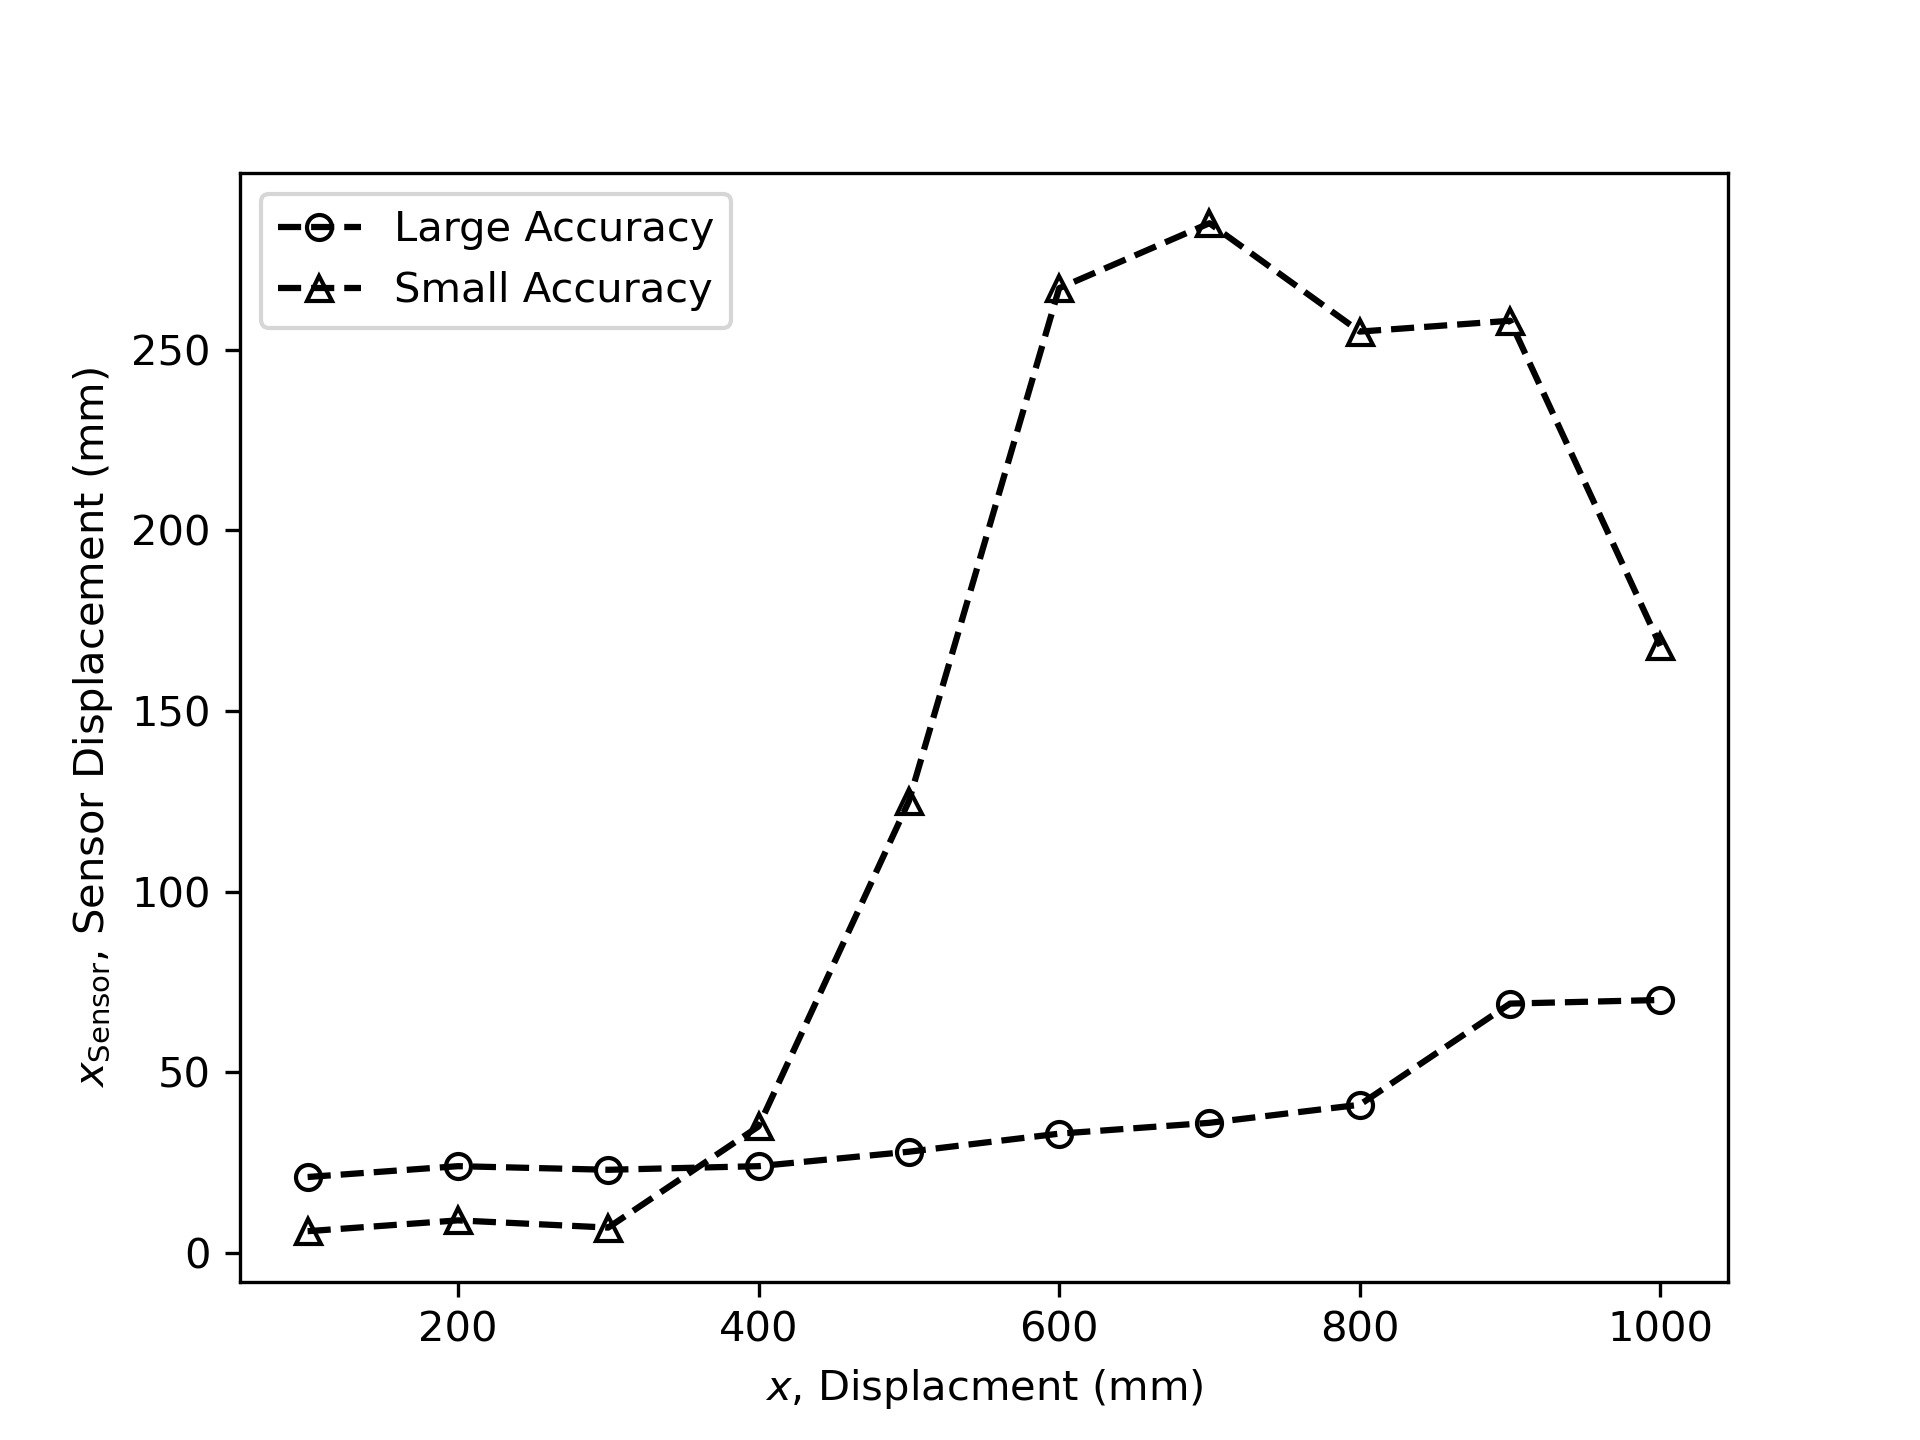
\includegraphics[width=0.6\linewidth]{matplotlib/Q3acc.png}
    \caption{Accuracy and repeatability of the sensor as a function of target displacement for each target size}
    \label{fig:Q3acc}
\end{figure}

\begin{figure}[h]
    \centering
    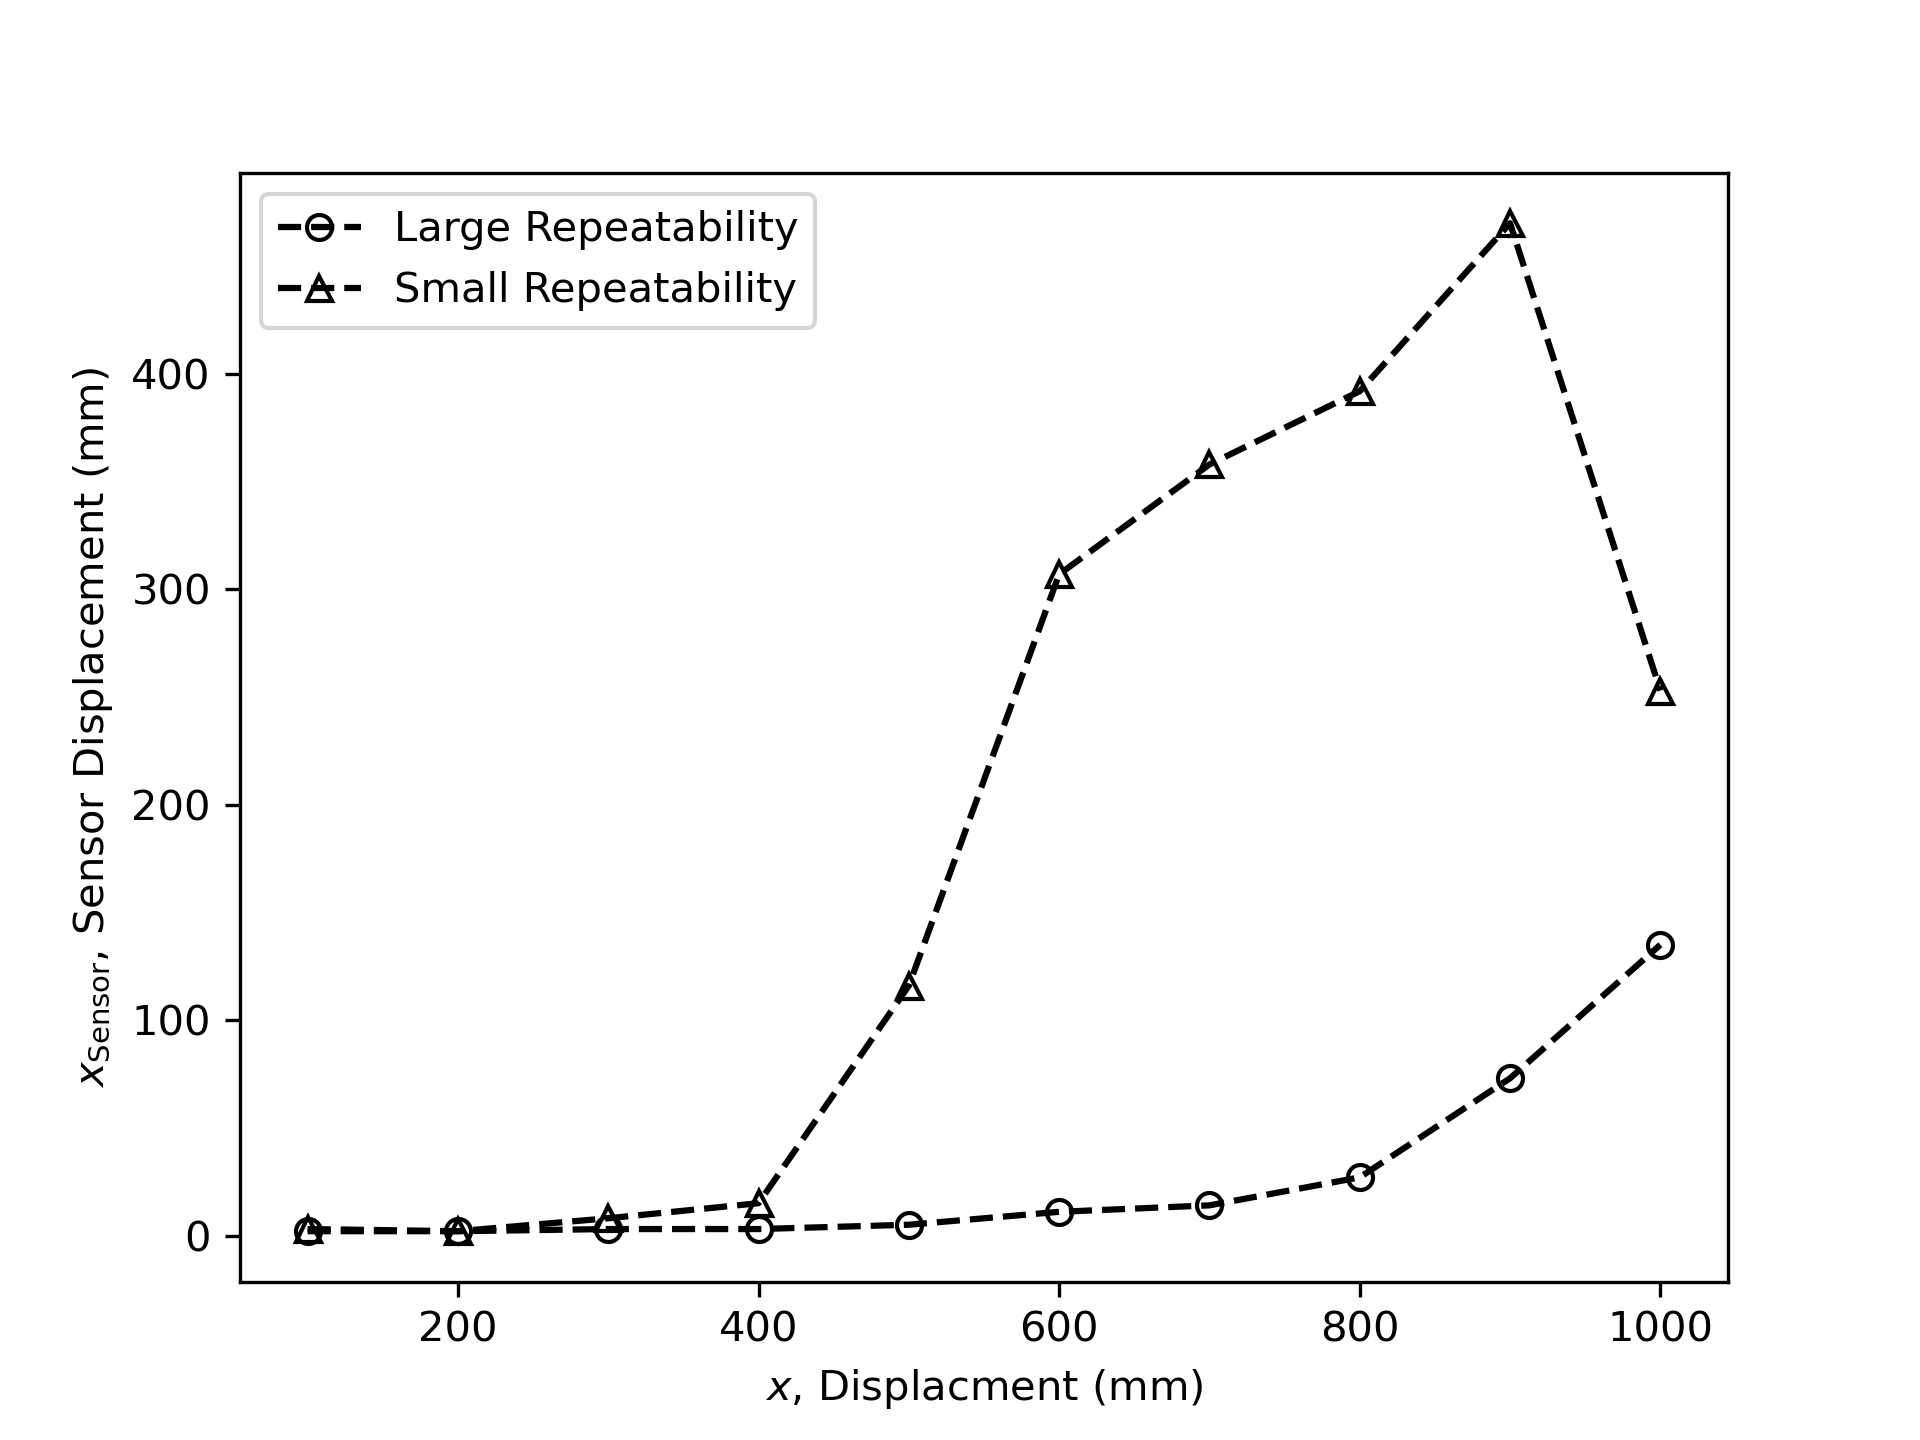
\includegraphics[width=0.6\linewidth]{matplotlib/Q3rep.png}
    \caption{Repeatability of the sensor as a function of target displacement for each target size}
    \label{fig:Q3rep}
\end{figure}

\FloatBarrier
\subsection{}
% b) How does the accuracy of the sensor change with target size? Why?

The accuracy of the sensor increases with target size and decreases with target displacement. This is because the larger target size is easier to detect.
Observing the target signal strengths, the large target had a higher signal strength than the small target for all displacements. Status 2 was reached
at a lower displacement for the smaller target than the larger target, meaning the sensor had less confidence in the reading provided.

In Fig. \ref{fig:Q3acc}, the accuracy of the smaller target was slightly higher than the larger target at 100mm, 200mm, and 300mm. This diverges
quickly as the displacement increases.  
\FloatBarrier
\section{}
% Assuming the accuracy of the tape measure is 1 mm and the accuracy of the 
% micrometer is 0.003 mm, calculate the total uncertainty in your measurements of b, 
% h and L (use 95% confidence interval for all uncertainty calculations in this lab.)
% stdev	T-INV	P_x	B_x	U_x
% Description	mm		mm	mm	mm
% Distance from centre of strain gauge to weight hanger, L	0.4	2.7764	0.5	1	1
% Width of beam, b	0.001	2.7764	0.001	0.003	0.003
% Height of beam, h	0.002	2.7764	0.002	0.003	0.004

\begin{table}[h]
    \centering
    \caption{Uncertainty in measurements of $b$, $h$, and $L$}
    \label{tab:Q4Uncertainty}
    \begin{tabular}{cccccc}
        \toprule
        Dimension & STDEV & $T_{\text{INV}}$ & $P_x$ & $B_x$ & $U_x$ \\
        & (mm) & & (mm) & (mm) & (mm) \\
        \midrule
        $L$ & 0.4 & 2.7764 & 0.5 & 1 & 1 \\
        $b$ & 0.001 & 2.7764 & 0.001 & 0.003 & 0.003 \\
        $h$ & 0.002 & 2.7764 & 0.002 & 0.003 & 0.004 \\
        \bottomrule
    \end{tabular}
\end{table}

A sample calculation of the uncertainty in $L$ is shown below. The uncertainty in $b$ and $h$ are calculated in a similar manner.

Using Excel's \texttt{STDEV.S} function applied to Table \ref{tab:Q2BeamMeasurements}, \texttt{T.INV} function with $\alpha = 0.05$ and $n = 5$, 
the precision uncertainty $P_x$ is calculated as:
\begin{align*}
    P_x &= \frac{S_x}{\sqrt{n}} \times t_{\alpha/2, n-1} \\
    &= \frac{0.4}{\sqrt{5}} \times 2.7764 \\
    &= \qty{0.5}{mm}
\end{align*}

The bias uncertainty $B_x$ was given to be 1 mm. The total uncertainty $U_x$ is calculated as:
\begin{align*}
    U_x &= \sqrt{P_x^2 + B_x^2} \\
    &= \sqrt{(0.5)^2 + (1)^2} \\
    &= \boxed{\qty{1}{mm}}
\end{align*}




\section{}
% Calculate the total uncertainty in the theoretical strain when the 1 kg weight was 
% applied to the beam. The uncertainty in the weight is 5 g and the uncertainty in the 
% modulus of elasticity is 1 GPa.

The relevant equations are:
\begin{align*}
    M &= mgL \\
    \sigma &= \frac{Mh}{2I} \\
    I &= \frac{bh^3}{12} \\
    \epsilon &= \frac{\sigma}{E}
\end{align*}

Combining these equations, we get:
\begin{align*}
    \epsilon &= \frac{6mgL}{b h^2 E} \\
\end{align*}

Computing the partials,
\begin{align*}
    \frac{\partial \epsilon}{\partial m} &= \frac{6gL}{b h^2 E} \\
    \frac{\partial \epsilon}{\partial L} &= \frac{6mg}{b h^2 E} \\
    \frac{\partial \epsilon}{\partial b} &= -\frac{6mgL}{b^2 h^2 E} \\
    \frac{\partial \epsilon}{\partial h} &= -\frac{12mgL}{b h^3 E} \\
    \frac{\partial \epsilon}{\partial E} &= -\frac{6mgL}{b h^2 E^2} \\
\end{align*}

Evaluating the partials times the uncertainty in each variable,
\begin{align*}
    \frac{\partial \epsilon}{\partial m} \delta m &=  4.17 \times 10^{-7} \\
    \frac{\partial \epsilon}{\partial L} \delta L &=  4.60 \times 10^{-7} \\
    \frac{\partial \epsilon}{\partial b} \delta b &=  2.12 \times 10^{-8} \\
    \frac{\partial \epsilon}{\partial h} \delta h &=  4.96 \times 10^{-8} \\
    \frac{\partial \epsilon}{\partial E} \delta E &=  1.21 \times 10^{-6} \\
\end{align*}

The total uncertainty is the RSS of the partials times the uncertainty in each variable:
\begin{align*}
    \delta \epsilon &= \sqrt{(4.17\times 10^{-7})^2 + (4.60\times 10^{-7})^2 + (2.12\times 10^{-8})^2 + (4.96\times 10^{-8})^2 + (1.21\times 10^{-6})^2} \\
    &= \boxed{\pm\qty{1.36E-6}{}}
\end{align*}

The calculations were handled by Matlab, and the code is shown below:
\begin{lstlisting}[language=Matlab]
clc; clear; close all;
syms m g L b h E  

epsilon = 6*m*g*L/(b*h^2*E)
 
delEdelm = diff(epsilon, m)
delEdelL = diff(epsilon, L)
delEdelb = diff(epsilon, b)
delEdelh = diff(epsilon, h)
delEdelE = diff(epsilon, E)

delEdelm_delta_m = double(subs(delEdelm, [m g L b h E], [1 9.81 0.2027 0.012811 0.0127256 68.9*10^9]) * 0.005)
delEdelL_delta_L = double(subs(delEdelL, [m g L b h E], [1 9.81 0.2027 0.012811 0.0127256 68.9*10^9]) * 1.11654678249935/1000)
delEdelb_delta_b = double(subs(delEdelb, [m g L b h E], [1 9.81 0.2027 0.012811 0.0127256 68.9*10^9]) * 0.00325628602303491/1000)
delEdelh_delta_h = double(subs(delEdelh, [m g L b h E], [1 9.81 0.2027 0.012811 0.0127256 68.9*10^9]) * 0.00378200336150775/1000)
delEdelE_delta_E = double(subs(delEdelE, [m g L b h E], [1 9.81 0.2027 0.012811 0.0127256 68.9*10^9]) * 1*10^9)

delE_delta_E = sqrt(delEdelm_delta_m^2 + delEdelL_delta_L^2 + delEdelb_delta_b^2 + delEdelh_delta_h^2 + delEdelE_delta_E^2)
\end{lstlisting}
\section{}
% Determine the total uncertainty in Δ𝐸0 only for the full bridge when the 1 kg weight 
% was used: As shown in Eq 2, Δ𝐸0
% is the voltage difference measured by the Arduino 
% divided by the gain. Note that 𝐸w and 𝐸nw are both measured by the same device 
% (the Arduino) and thus 𝐸w and 𝐸nw are not independent measurements. This is a 
% special (but common) case in uncertainty analysis. Note that in this case, a 
% systematic bias in the voltage measurement creates no error in the difference 
% between the voltages (i.e., if the Arduino always measured 10 mV too low it would 
% result in no error in the voltage difference). However, other sources of bias
% (resolution or linearity) could still cause errors. In this case, resolution is the largest 
% bias uncertainty and would have a maximum value equal to the resolution of the 
% Arduino (3.3 V/2
% 10). There would also be precision uncertainty in the 
% measurement of the voltage difference (Δ𝐸w). Thus, calculate the total uncertainty 
% in Δ𝐸w then use the propagation of uncertainty to find the total uncertainty in Δ𝐸0
% assuming the uncertainty in the gain is 1%.

\subsection{Uncertainty in $\Delta E_w$}
% stdev	T-INV	P_x	B_x	U_x
% Description	mm		mm	mm	mm
% delta Ew	0.002683282	2.5706	0.0028	0.003222656	0

\begin{table}[h]
    \centering
    \caption{Uncertainty in $\Delta E_w$}
    \label{tab:Q5UncertaintyDeltaEw}
    \begin{tabular}{cccccc}
        \toprule
        Dimension & STDEV & T-INV & $P_x$ & $B_x$ & $U_x$ \\
        & (V) & & (V) & (V) & (V) \\
        \midrule
        $\Delta E_w$ & 2.683E-03 & 2.5706 & 2.8E-03 & 3.223E-03 & 4.3E-03 \\
        \bottomrule
    \end{tabular}
\end{table}

Again, standard deviation is calculated using Excel's \texttt{STDEV.S} function. T-INV is calculated using Excel's \texttt{T.INV} function with $\alpha = 0.05$ and $n = 6$. 
The precision uncertainty $P_x$ is calculated as:
\begin{align*}
    P_x &= \frac{S_x}{\sqrt{n}} \times t_{\alpha/2, n-1} \\
    &= \frac{2.683E-03}{\sqrt{6}} \times 2.5706 \\
    &= \qty{2.8E-03}{V}
\end{align*}

The bias uncertainty $B_x$ is the resolution, 
\begin{align*}
    B_x &= \frac{3.3}{2^{10}} \\
    &= \qty{3.223E-03}{V}
\end{align*}

The total uncertainty $U_x$ is calculated as:
\begin{align*}
    U_x &= \sqrt{P_x^2 + B_x^2} \\
    &= \sqrt{(2.8\times 10^{-3})^2 + (3.223 \times 10^{-3})^2} \\
    &= \boxed{\qty{4.3E-03}{V}}
\end{align*}

\subsection{Uncertainty in $\Delta E_0$}
The equation for $\Delta E_0$ is given by:
\begin{align*}
    \Delta E_0 &= \frac{\Delta E_w}{G} \\
    &= \frac{4.3 \times 10^{-3}}{2.09} \\
    &= \boxed{\qty{2.06E-03}{V}}
\end{align*}

Calculating the partials,
\begin{align*}
    \frac{\partial \Delta E_0}{\partial \Delta E_w} &= \frac{1}{G} \\
    \frac{\partial \Delta E_0}{\partial G} &= -\frac{\Delta E_w}{G^2}
\end{align*}

Calculating the partials times the uncertainty (the nominal value for $\Delta E_w$ is 1.160 V),
\begin{align*}
    \frac{\partial \Delta E_0}{\partial \Delta E_w} \delta \Delta E_w &=  \frac{1}{3000} \times 4.3 \times 10^{-3} \\
    & = 1.4\times 10^{-6} \\
    \frac{\partial \Delta E_0}{\partial G} \delta G &=  -\frac{1.160}{3000^2} \times 1 \times 3000 \\
    & = -3.9\times 10^{-6}
\end{align*}

The total uncertainty is the RSS of the partials times the uncertainty in each variable:
\begin{align*}
    \delta \Delta E_0 &= \sqrt{(1.4\times 10^{-6})^2 + (-3.9\times 10^{-6})^2} \\
    &= \boxed{\qty{3.6E-5}{V}}
\end{align*}
\section{}
% Determine the total uncertainty in the strain only for the full bridge when the 1 kg 
% weight was used. It is best to do this by calculating the total uncertainty in each 
% variable and then find the total uncertainty in the strain via propagation of errors. 
% The uncertainty in the strain gauge factor is 0.02 and the uncertainty in the input 
% voltage is 0.5%. 

The equation for strain for the full bridge is:
\begin{align*}
    \epsilon &= \frac{\Delta E_0}{F_g V_{\text{in}}} 
\end{align*}

The partials are:
\begin{align*}
    \frac{\partial \epsilon}{\partial \Delta E_0} &= \frac{1}{F_g V_{\text{in}}} \\
    \frac{\partial \epsilon}{\partial F_g} &= -\frac{\Delta E_0}{F_g^2 V_{\text{in}}} \\
    \frac{\partial \epsilon}{\partial V_{\text{in}}} &= -\frac{\Delta E_0}{F_g V_{\text{in}}^2} \\
\end{align*}

Evaluating the partials times the uncertainty of each variable is shown in Table \ref{tab:Q7UncertaintyEpsilon}. For example,
\begin{align*}
    \frac{\partial \epsilon}{\partial \Delta E_0} \delta \Delta E_0 &=  \frac{1}{2.09 \times 3.3} \times 5.65 \times 10^{-4} \\
    & = 5.21\times 10^{-6}
\end{align*}
\begin{table}[h]
    \centering
    \caption{Partials times uncertainty for variables in $\epsilon$}
    \label{tab:Q7UncertaintyEpsilon}
    \begin{tabular}{cccc}
        \toprule
        Variable & Nominal Value & Uncertainty & $\frac{\partial \epsilon}{\partial x_i} \delta x_i$ \\
        \midrule
        $\Delta E_0$ & 5.65E-04 & 3.59E-05 & 5.21E-06 \\
        $F_g$ & 2.09 & 0.02 & -7.83E-07 \\
        $V_{\text{in}}$ & 3.3 & 0.017 & -1.35E-06 \\
        \bottomrule
    \end{tabular}
\end{table}

The total uncertainty in $\epsilon$ is the RSS of the partials times the uncertainty in each variable:
\begin{align*}
    U_{x} &= \sqrt{\left(\frac{\partial \epsilon}{\partial \Delta E_0} \delta \Delta E_0\right)^2 + \left(\frac{\partial \epsilon}{\partial F_g} \delta F_g\right)^2 + 
    \left(\frac{\partial \epsilon}{\partial V_{\text{in}}} \delta V_{\text{in}}\right)^2} \\
    &= \sqrt{(5.21\times 10^{-6})^2 + (-7.83\times 10^{-7})^2 + (-1.35\times 10^{-6})^2} \\
    &= \boxed{5.4 \times 10^{-6}}
\end{align*}

% \newpage
% %\bibliographystyle{IEEEtran}
% %\bibliography{citations.bib}
% %\bibliography{}

\newpage
\appendix
\renewcommand\thefigure{\thesection.\arabic{figure}}    
\renewcommand\thetable{\thesection.\arabic{table}}
\newpage
\section{Appendix: Displacement Table of Potentiometer}
\label{sec:appendix-potentiometer-displacement-table}

% Up 1	Down 1	Up 2	Down 2	Up 3	Down 3
% 0		-0.16		-0.16		-0.16
% 3.64	3.61	3.61	3.61	3.65	3.61	3.65
% 7.64	7.69	7.69	7.69	7.69	7.69	7.73
% 11.64	11.69	11.69	11.69	11.66	11.66	11.66
% 15.64	15.70	15.66	15.66	15.66	15.66	15.70
% 19.64	19.65	19.65	19.61	19.61	19.65	19.61
% 23.64	23.66	23.62	23.66	23.62	23.66	23.62
% 27.64	27.70	27.66	27.66	27.66	27.70	27.66
% 31.64	31.67	31.63	31.67	31.63	31.67	31.67
% 39.1	38.98		38.98		38.98	


\begin{table}[h]
    \centering
    \caption{Displacement table of potentiometer}
    \label{tab:appendix-potentiometer-displacement-table}
    \begin{tabular}{cccccc}
        \hline
        Caliper Reading & Up 1 & Down 1 & Up 2 & Down 2 & Up 3 \\
        (mm) & (mm) & (mm) & (mm) & (mm) & (mm) \\
        \midrule
        0.00 & & -0.16 & & -0.16 & \\
        3.64 & 3.61 & 3.61 & 3.61 & 3.65 & 3.61 \\
        7.64 & 7.69 & 7.69 & 7.69 & 7.69 & 7.73 \\
        11.64 & 11.69 & 11.69 & 11.69 & 11.66 & 11.66 \\
        15.64 & 15.70 & 15.66 & 15.66 & 15.66 & 15.70 \\
        19.64 & 19.65 & 19.65 & 19.61 & 19.61 & 19.65 \\
        23.64 & 23.66 & 23.62 & 23.66 & 23.62 & 23.66 \\
        27.64 & 27.70 & 27.66 & 27.66 & 27.66 & 27.70 \\
        31.64 & 31.67 & 31.63 & 31.67 & 31.63 & 31.67 \\
        39.10 & 38.98 & & 38.98 & & 38.98 \\
        \hline
        \hline
    \end{tabular}
\end{table}

\FloatBarrier
\phantom{a}

\newpage
\section{Appendix: Hall Effect Sensor Displacement Table}
\label{sec:appendix-hall-effect-sensor-displacement-table}
% Caliper reading referenced to zero displacement	First measurement	Second measurement	Third measurement	Fourth measurement	Fifth measurement
% (mm)	(mm)	(mm)	(mm)	(mm)	(mm)
% 0.00	-0.01	-0.01	0.00	-0.01	-0.01
% 0.38	0.40	0.41	0.40	0.40	0.39
% 0.88	0.86	0.88	0.87	0.86	0.85
% 1.38	1.36	1.34	1.38	1.37	1.37
% 1.88	1.92	1.92	1.89	1.89	1.87
% 2.38	2.40	2.41	2.41	2.41	2.40
% 2.88	2.83	2.90	2.87	2.83	2.86

\begin{table}[h]
    \centering
    \caption{Hall effect sensor displacement table}
    \label{tab:appendix-hall-effect-sensor-displacement-table}
    \begin{tabular}{cccccc}
        \hline
        Caliper Reading & First Measurement & Second Measurement & Third Measurement & Fourth Measurement & Fifth Measurement \\
        (mm) & (mm) & (mm) & (mm) & (mm) & (mm) \\
        \midrule
        0.00 & -0.01 & -0.01 & 0.00 & -0.01 & -0.01 \\
        0.38 & 0.40 & 0.41 & 0.40 & 0.40 & 0.39 \\
        0.88 & 0.86 & 0.88 & 0.87 & 0.86 & 0.85 \\
        1.38 & 1.36 & 1.34 & 1.38 & 1.37 & 1.37 \\
        1.88 & 1.92 & 1.92 & 1.89 & 1.89 & 1.87 \\
        2.38 & 2.40 & 2.41 & 2.41 & 2.41 & 2.40 \\
        2.88 & 2.83 & 2.90 & 2.87 & 2.83 & 2.86 \\
        \hline
    \end{tabular}
\end{table}


\end{document}